%!TEX root = ../msc_thesis.tex

\chapter{Theoretical Framework}
\label{ch:theory}

%%%%%%%%%%%%%%%%%%%%%%%%%%%%%%%%%%%%%%%%%%%%%%%%%%%%%%%%%%%%%%%%%%%%%%%%%%%%%%%%%%%%%%%%%%
%%%%%%%%%%%%%%%%%%%%%%%%%%%%%%%%%%%%%%%%%%%%%%%%%%%%%%%%%%%%%%%%%%%%%%%%%%%%%%%%%%%%%%%%%%
%%% Related work
%%%%%%%%%%%%%%%%%%%%%%%%%%%%%%%%%%%%%%%%%%%%%%%%%%%%%%%%%%%%%%%%%%%%%%%%%%%%%%%%%%%%%%%%%%
%%%%%%%%%%%%%%%%%%%%%%%%%%%%%%%%%%%%%%%%%%%%%%%%%%%%%%%%%%%%%%%%%%%%%%%%%%%%%%%%%%%%%%%%%%

\section{Related work}

As mentioned before, Bayesian Artificial Neural Networks date back to late 1980s and early 1990s. These first approaches focused on Markov Chain Monte Carlo (MCMC) as the main method get samples of the posterior distribution of the parameters. Lately, there's been more work in the area, such as the Probabilistic Backpropagation algorithm developed by \citeauthor{hernandez2015probabilistic}, which relies on one-dimensional Gaussian distributions that approximate the marginal posterior distribution of the weights on each iteration of backpropagation \cite{hernandez2015probabilistic}. There is also the work by \citeauthor{graves2011practical}, based on variational inference to approximate the posterior distribution of the parameters \cite{graves2011practical}. These methods, however, do not scale well to very big network architectures and datasets; and they also have the disadvantage that they only work with multi-layer perceptron architectures, making them impossible to use with more recent architectures such as Convolutional Neural Networks (CNNs) or Recurrent Neural Networks (RNNs).

Recently, \citeauthor{gal2015dropout1} showed that a neural network with arbitrary depth, with dropout applied before each weight layer, is equivalent to the variational approximation to a deep Gaussian process. This is because the loss function minimizes the Kullback-Leibler divergence between an approximate distribution and the posterior of a deep Gaussian process \cite{gal2015dropout1}. This means that we can get uncertainty estimates with the models already trained with dropout without changing anything during training, the only difference comes at prediction time in which instead of doing a single forward pass and multiply each layer by a weight proportional to dropout probability, we just do several forward passes with dropout. They also showed in \cite{gal2015modern} that stochastic regularization techniques in arbitrary neural models can be seen as approximate variational inference in Bayesian Neural Networks.

This work is further extended by the same authors and they showed that the same ideas of dropout as a Bayesian approximation can be used in CNNs \cite{gal2015bayesian}. In particular, the showed that dropout can be seen as approximate variational inference in Bayesian Neural Networks, thus permitting the use of operations such as convolution and pooling in probabilistic models. The implementation is reduced to performing dropout after each convolution layer at training, and by performing several stochastic forward passes through the model (same idea as before). These stochastic forward passes are referred to as Monte Carlo (MC) dropout. Dropout is not usually performed after convolutional layers because it does not seem to give any benefits, but \citeauthor{gal2015bayesian} show empirically that MC-dropout can help with overfitting.

The work on CNNs is then used in an Active Learning environment, where the goal is to label images intelligently so that a model has good performance with a lower number of training examples \cite{Gal2016Active}. Deep learning poses several difficulties when used in an Active Learning setting because, first, small amounts of data need to be handled; and second, many Active Learning acquisition functions rely on model uncertainty, which is rarely represented in Deep Learning. \citeauthor{Gal2016Active} are able to achieve 5\% test error on the MNIST dataset with only 295 labeled images without, and 1.64\% test error with 1000 labeled images. They compare five different acquisition functions: choosing images that maximize the predictive entropy (Max Entropy); the ones that maximize the mutual information between predictions and model posterior (BALD); the ones that maximize the Variation Ratios; the ones that maximize mean standard deviation; and random acquisition (baseline). They also compare it with deterministic CNNs which, like the Bayesian CNN, produce a probability vector which can be used with the acquisition functions, but the Bayesian models, propagating uncertainty throughout the model, attain higher accuracy early on, and converge to a higher accuracy overall.

The dropout variational approach can also be used in Recurrent Neural Networks (RNNs), as shown by \citeauthor{gal2016theoretically} in \cite{gal2016theoretically}. In this paper, the authors give insight on how to use dropout with RNNs (something seldom done) and apply it on LSTM and GRU models, outperforming existing techniques in language modeling with the Penn Treebank dataset.

An example of how the uncertainties provided by Bayesian Neural Networks can be used, is shown by \citeauthor{li2017dropout} in \cite{li2017dropout}. They use adversarial examples and check if they can be told apart by examining the uncertainty representation of the dropout models. The deterministic Neural Networks produce over-confident predictions on these adversarial samples (they predict the wrong label very confidently), while dropout models, though producing wrong labels, are very uncertain about their predictions. They finish by stating that their results suggest that assessing the uncertainty of classification models can be used to identify adversarial examples, but much more research is needed to solve the difficulties faced with adversarial inputs.

The research on adversarial examples is continued by \citeauthor{rawat2017adversarial}, who study different Bayesian approaches (Bayes by Backprob (BBB), Probabilistic Backpropagation (PBP), Variational Matrix Gaussian (VMG) and MC-Dropout) and the uncertainty provided by the models, and prove that these models exhibit increased uncertainty when under attack \cite{rawat2017adversarial}. They state that all of the architectures in their study are Multi-Layer Perceptron, which do not scale for high dimensional colored images, with the exception of MC-Dropout, and therefore, a detailed study for MC-Dropout is required to demonstrate the applicability of model uncertainty for adversarial detection on various state-of-the-art attacks.

%%%%%%%%%%%%%%%%%%%%%%%%%%%%%%%%%%%%%%%%%%%%%%%%%%%%%%%%%%%%%%%%%%%%%%%%%%%%%%%%%%%%%%%%%%
%%%%%%%%%%%%%%%%%%%%%%%%%%%%%%%%%%%%%%%%%%%%%%%%%%%%%%%%%%%%%%%%%%%%%%%%%%%%%%%%%%%%%%%%%%
%%%
%%%%%%%%%%%%%%%%%%%%%%%%%%%%%%%%%%%%%%%%%%%%%%%%%%%%%%%%%%%%%%%%%%%%%%%%%%%%%%%%%%%%%%%%%%
%%%%%%%%%%%%%%%%%%%%%%%%%%%%%%%%%%%%%%%%%%%%%%%%%%%%%%%%%%%%%%%%%%%%%%%%%%%%%%%%%%%%%%%%%%

\section{Machine learning}

Machine learning is a set of methods used to learn patterns in data, and then use these patterns to make predictions about new unseen data, or to take other decisions \cite{murphy2012machine}. With the amount of data available nowadays, it has become a fruitful and demanded field in many areas. Machine learning has exploded lately mainly thanks to the advanced in computing power, without which most of modern techniques wouldn't be feasible.

Machine learning is usually divided in two areas: supervised learning and unsupervised learning. The former involves building a model to predict a response variable from certain explanatory variables (or covariates); while the latter involves a set of variables without a response: one wishes to learn relationships and structure of the data.

An example of supervised learning is to estimate the income of a home from a set of variables such as zip code, size of home, number of cars they own, etc; and an example of unsupervised learning is to find groups of homes that naturally come up in the data, such that there is high similarity within each group and little between groups. In this work, only supervised learning is presented and studied.

As previously mentioned, in supervised learning we have a response variable denoted as vector $y$ with $n$ elements, and each covariate is denoted by $x^{(k)} \in \mathbb{R}^n$ for $k$ from 1 to $p$. All covariates can be summarized in notation in a single data matrix $X \in \mathbb{R}^{n \times p}$. It is assumed that there exists a relationship between $y$ and $X$, which can be written as

\begin{equation}
  \label{eq:general_learning_model}
  Y = f(X) + \varepsilon
\end{equation}

where $f$ is a fixed but unknown function and $\varepsilon$ is a random error term, independent from $X$ and with zero mean \cite[p.~16]{james2013introduction}. We usually want to estimate function $f$, either prediction or inference, and we do it with an estimate $\hat{f}$ \cite[p.~17]{james2013introduction}.
In this work, we will focus on the prediction goal.
The estimate $\hat{f}$ can be chosen from a wide family of models, such as a linear regression model, a general additive model, a neural network, etc., and the goal is for $\hat{f}$ have as little generalization error as possible. This is done using a training set of data, denoted $\mathcal{L} = \left\{ (x_1, y_1), ..., (x_n, y_n) \right\}$, and an error or loss function that we wish to minimize.

For example, in the linear regression case, it is common to minimize the squared error function

$$
  \hat{f} = \argmin_{f \in \mathcal{F}} \frac{1}{n} \sum_{i = 1}^n{ ( y_i - f(x_i) ) ^ 2},
$$

where $\mathcal{F}$ is the family of functions of the form $f(X) = X\theta$ with $\theta \in \mathbb{R}^p$. Thus, $\hat{f}(X) = X \hat{\theta}$, where $\hat{\theta}$ minimizes the error function.

The linear regression model belongs to a type of methods called \textbf{parametric methods}, in which we first make an assumption about the functional form of $f$, and then train the model by choosing the parameters that minimize a previously selected error function \cite[p.~21]{james2013introduction}. In the case of linear regression, the form of $f$ is assumed to be $f(X) = X\theta$, and the parameters chosen are the elements of the $\hat{\theta}$ vector that minimize the squared error function of the model.

An approach to the estimation of parameters that is different to the concept of error function minimization, and one that is also more general, is the one of \textbf{maximum likelihood estimation}.
This is a probabilistic approach in which we assume certain probability distribution for the data.
In the case of linear regression, if we assume that the error term in \ref{eq:general_learning_model} has a Gaussian distribution such that $\varepsilon \sim \normaldist{0}{\sigma^2}$, then $y_i \sim \normaldist{X \theta}{\sigma^2}$; and if we also assume that the observations $y_i$ for $i$ from 1 to $n$ come from a random sample and are, thus, independent of each other, then the log-probability of the sample is

\begin{equation}
  \label{eq:gaussian_likelihood}
  L(\theta) = \sum_{i = 1}^n \log \normalfunc{y_i}{X \theta}{\sigma^2},
\end{equation}

where $\normalfunc{x_i}{\mu}{\sigma^2}$ denotes the density function of a Gaussian random variable with mean $\mu$ and variance $\sigma^2$. The \textbf{principle of maximum likelihood} states that the values for $\theta$ should be chosen so that the observed probability of the random sample is the highest, i.e., so that they maximize equation \ref{eq:gaussian_likelihood} \cite[p.~31]{friedman2001elements}.
With some algebra, it is fairly easy to see that maximizing equation \ref{eq:gaussian_likelihood} is equivalent to minimizing the squared error loss.

In the case of a binary classification problem, assuming that $y_i$ follows a Bernoulli distribution, such that the probability of $y_i$ of being 1 is $p_i(\theta)$, where $\theta$ is the parameter that indexes the probability, then the likelihood function in this case is $\prod_{i = 1}^n  p_i(\theta)^{y_i}\left(1 - p_i(\theta) \right)^{1 - y_i}$ and thus, the log-likelihood is

$$
  L(\theta) = \sum_{i = 1}^n \left[ y_i \log\left( p_i(\theta) \right) + (1 - y_i) \log \left( 1 - p_i(\theta) \right) \right].
$$

Another approach to the learning problem is the \textbf{Bayesian approach}, in which we first assume a prior distribution on the parameters $\theta$ and we update our knowledge about them with data $X$. That is, we first quantify the knowledge that we may have about $\theta$ using a prior distribution $\prob{\theta}$ and then compute the posterior distribution of $\theta$ given $X$ using Bayes' theorem as such

\begin{equation}
  \label{eq:bayes_theorem}
  \prob{\theta | X} = \frac{\prob{X | \theta} \prob{\theta}}{\prob{X}} = \frac{\prob{X | \theta} \prob{\theta}}{\int \prob{X | \theta} \prob{\theta} d\theta}.
\end{equation}

The posterior distribution represents the knowledge that we have about $\theta$ after we have seen the data and is a compromise between our prior beliefs and the data. The multiplier $\prob{X | \theta}$ is called the likelihood, and is the probability of the data given the parameters.

Since the denominator of equation \ref{eq:bayes_theorem} does not depend on $\theta$ because it is only a normalizing constant, it is just usually described as a proportion

\begin{equation}
  \label{eq:bayes_theorem_prop}
    \prob{\theta | X} \propto \prob{X | \theta} \prob{\theta}.
\end{equation}

This posterior distribution is also used to predict the values of unseen data. Let $x^*$ be a vector of covariates for which we want to make a prediction $\hat{y}^*$, then we use the \textbf{posterior predictive distribution}, defined as

$$
  \prob{x^* | X} = \int \prob{x^* | \theta} \prob{\theta | X} d\theta.
$$

Note that this posterior distribution is, as it name implies, a distribution; i.e., it is not a single prediction but a whole bunch of predictions, quantified by how likely each value is to be. If we wanted a point prediction $\hat{y}^*$ for $x^*$ then we could take the expected value of the posterior predictive distribution such that

$$
  \hat{y}^* = \mathbb{E}_{x^* | X} \left[ \prob{x^* | X} \right].
$$

There are other possible point estimates such as the median, or the maximum a posteriori (MAP) estimate, but we will not study them in detail.

We can illustrate all these concepts in the context of logistic regression. Suppose that we have $n$ observations of a binary response variable $y \in \left\{0, 1\right\}^n$ and two continuous covariates $x^{(1)}, x^{(2)} \in \mathbb{R}^n$. First, we will a build a linear classifier with the frequentist approach, that is, with the maximum likelihood approach; then, we will transform this into a simple learning problem in which we try to minimize a loss function; and finally, we will see how the Bayesian approach works here.

If we wanted to build a linear classifier from our two covariates, we would run into a problem because the response variable only takes the values $0$ and $1$, and a linear model of the form $\mu(x_i) = \theta_0 + \theta_1 x_i^{(1)} + \theta_2 x_i^{(2)}$ is not bounded, so it is a better idea to model the probability of a feature vector of belonging to each class.
This way, $y_i$ is a random variable that follows a Bernoulli distribution with parameter $p_i$, where $p_i$ is the probability of $y_i$ being 1.
The range of $f$ as a linear model is $\mathbb{R}$, so we must map it to the $\left[ 0,1 \right]$ space in which probabilities live, and it can be done with what is called a \textbf{link function}. The \textbf{logistic sigmoid function} $\sigma \left( \cdot \right)$ is a widely used link function for this type of problems \cite[p.~114]{christopher2006pattern}. It is defined as

$$
  \sigma(w) = \frac{e^w}{1 + e^w} = \frac{1}{1 + e^{-w}}.
$$

It is easy to see that $\lim_{w \to -\infty} \sigma(w) = 0$ and $\lim_{w \to \infty} \sigma(w) = 1$. There is more reasoning behind the logistic sigmoid function, and some of it has to be that it belongs to the exponential family of functions. To see more details about this, see \cite{christopher2006pattern}.

Another possible link function is the \textbf{probit function}, defined as the inverse of the cumulative distribution function of a Gaussian random variable \cite[p.~296]{friedman2001elements}. That is, $\sigma(w) = \Phi^{-1}\left( x \right)$,
where

$$
  \Phi(w) = \int_{-\infty}^w \frac{1}{\sqrt{2 \pi}} \exp{\left( -\frac{x^2}{2} \right)} dx
$$

is the Gaussian cumulative distribution function. There are some differences in the theory and behavior of the logistic and the probit functions, but in practice they hardly make any substantial difference. Henceforth, we will use the logistic function as a link function for binary classification problems.

So, we know that $\sigma \left( \cdot \right)$ maps from $\mathbb{R}$ to $\left[ 0,1 \right]$, but we don't know exactly how to relate this to our original problem which is to build a linear classifier using the vectors $x^{(1)}$ and $x^{(2)}$. Using  $\sigma \left( \cdot \right)$, we can define the probability of $y_i$ of belonging to class $1$ given features $x_i^{(1)}$ and $x_i^{(2)}$, summarized as $x_i$, as

$$
  \prob{y_i = 1 | x_i, \theta} = \sigma(\theta_0 + \theta_1 x_i^{(1)} + \theta_2 x_i^{(2)}) = \frac{1}{1 + e^{-\left( \theta_0 + \theta_1 x_i^{(1)} + \theta_2 x_i^{(2)} \right)}},
$$

and thus

$$
  \prob{y_i = 0 | x_i, \theta} = 1 - \prob{y_i = 1 | x_i} = \frac{1}{1 + e^{\theta_0 + \theta_1 x_i^{(1)} + \theta_2 x_i^{(2)}}}.
$$

So, $y_i$ is fully described as a Bernoulli distribution with parameter $p_i =\prob{y_i = 1 | x_i, \theta}$. As we previously mentioned, the likelihood of $n$ observations is

$$
  \prod_{i = 1}^n  p_i(\theta)^{y_i}\left(1 - p_i(\theta) \right)^{1 - y_i}
$$

and, in consequence, the log-likelihood of $n$ observations is

\begin{equation}
  \label{eq:log_likelihood_logistic_example}
  L(\theta) = \sum_{i = 1}^n \left[ y_i \log\left( p_i(\theta) \right) + (1 - y_i) \log \left( 1 - p_i(\theta) \right) \right],
\end{equation}

where $p_i(\theta) = \sigma(\theta_0 + \theta_1 x_i^{(1)} + \theta_2 x_i^{(2)})$.

So, the maximum likelihood estimator of $\theta = \left[ \theta_0, \theta_1, \theta_2 \right]^T$ is the vector $\hat{\theta}$ that maximizes $L(\theta)$ in equation \ref{eq:log_likelihood_logistic_example}; that is $\hat{\theta} = \argmax L(\theta)$.

Another way to see the problem of binary classification, is to simply see it as a learning problem in which we want to minimize a certain loss function. We now know that maximizing equation \ref{eq:log_likelihood_logistic_example} gives us the maximum likelihood estimate, but if we change the sign, then we have a loss function that we can minimize, and it's the exact same problem as before. But first, let's write the new loss function and try to understand the logic behind it. The new objective function, that we wish to minimize is

\begin{equation}
  \label{eq:logistic_example_loss_function}
  L(\theta) = - \sum_{i = 1}^n \left[ y_i \log\left( p_i(\theta) \right) + (1 - y_i) \log \left( 1 - p_i(\theta) \right) \right].
\end{equation}

Now, why is this an error function? If $y_i = 1$, then $1 - y_i = 0$, so the second term in the loss function vanishes and we have remaining $\log\left( p_i(\theta) \right)$. Now, if we assign a high value to $p_i(\theta)$, that is, close to 1, then $\log\left( p_i(\theta) \right) \approx 0$; but if we assign a low value to $p_i(\theta)$, that is, close to 0, then $\log\left( p_i(\theta) \right) \approx -\infty$, and so the overall loss function (don't forget that there's a minus sign at the beginning) tends to infinity. This means that when the real value of $y_i$ is 1 and we assign a low probability to it, the loss function is large, but if we assign a high probability to it, the loss function is small. The same reasoning works for when $y_i = 0$: if we assign a low probability, then the loss function is small, but if we assign a high probability, then the loss function is large. Hence, minimizing the loss function leads to choosing values of $\theta$ such that they yield a high probability to the cases when $y_i = 1$ and a low one when $y_i = 0$.

% There are other possible loss functions for this problem, such as the \textbf{hinge loss}

Now, let's move to the Bayesian approach to logistic regression. As before, we will assume that $y_i$ follows a Bernoulli distribution such that the probability of being 1 is $p_i(\theta) = \sigma(\theta_0 + \theta_1 x_i^{(1)} + \theta_2 x_i^{(2)})$, with $\sigma \left( \cdot \right)$ the logistic sigmoid function. In the Bayesian paradigm, parameter vector $\theta = \left[ \theta_0, \theta_1, \theta_2 \right]^T$ must have a joint prior distribution. As mentioned before, a good idea is to place a Gaussian distribution to it and, in this case, assume independence between the parameters, such that

$$
  \theta \sim \normaldist{\mu}{\frac{1}{\tau} I}
$$

where $\mu \in \mathbb{R}^3$, $\tau \in \mathbb{R}^+$ and $I$ is a $3 \times 3$ identity matrix. In this context, $\tau$ is the inverse of the variance, and is called the \textbf{precision}. Assuming $\mu = \left[ \mu_0, \mu_1, \mu_2 \right]^T$, then the prior distribution takes the following form

$$
  \prob{\theta} = \prod_{k = 0}^2 \sqrt{\frac{\tau}{2 \pi}} e^{- \tau \frac{\left( \theta_k - \mu_k \right)^2}{2}}.
$$

And, the likelihood is

$$
  \prob{X | \theta} = \prod_{i = 1}^n  p_i(\theta)^{y_i}\left(1 - p_i(\theta) \right)^{1 - y_i},
$$

so, following Bayes' theorem in equation \ref{eq:bayes_theorem_prop}, the posterior distribution is

$$
  \prob{\theta | X} =
    \frac
    {
      \left[ \prod_{i = 1}^n  p_i(\theta)^{y_i}\left(1 - p_i(\theta) \right)^{1 - y_i} \right]
      \left[ \prod_{k = 0}^2 \sqrt{\frac{\tau}{2 \pi}} e^{- \tau \frac{\left( \theta_k - \mu_k \right)^2}{2}} \right]
    }{
      \int \left[ \prod_{i = 1}^n  p_i(\theta)^{y_i}\left(1 - p_i(\theta) \right)^{1 - y_i} \right]
      \left[ \prod_{k = 0}^2 \sqrt{\frac{\tau}{2 \pi}} e^{- \tau \frac{\left( \theta_k - \mu_k \right)^2}{2}} \right] d\theta
    }.
$$

Unfortunately, the integral is not directly solvable, and that is the reason numerical methods are used. Most of them rely on the fact that the denominator is only a normalizing constant and only use the equation as a proportion

$$
  \prob{\theta | X} \propto
  \left[ \prod_{i = 1}^n  p_i(\theta)^{y_i}\left(1 - p_i(\theta) \right)^{1 - y_i} \right]
  \left[ \prod_{k = 0}^2 \sqrt{\frac{\tau}{2 \pi}} e^{- \tau \frac{\left( \theta_k - \mu_k \right)^2}{2}} \right].
$$

Methods to estimate the posterior include Markov Chain Monte Carlo (MCMC) methods such as Metropolis-Hastings or Hamiltonian Monte Carlo, and Variational Inference, discussed later in this document.


% En general, cuando uno entrena un modelo para predecir, no se desea minimizar el error de entrenamiento, sino el error de predicción, esto es, el error de cualquier observación futura $(X^0, Y^0)$. Esto quiere decir que se quiere minimizar el error esperado de predicción, definido como $\mathbb{E} \left[ L(\hat{f}(X^0), Y^0 ) \right]$.
%
% Debido a que se quiere minimizar el error esperado de predicción, es común separar el conjunto de datos $(X, Y)$ en dos, el conjunto de entrenamiento, presentado anteriormente como $\mathcal{L}$, y un \textit{conjunto de validación} o \textit{conjunto de prueba} denotado como $\mathcal{T}$. Para hacer esto, del conjunto original de datos, se toma una muestra aleatoria para entrenar (este es el conjunto de entrenamiento $\mathcal{L}$) y el resto es el conjunto de validación $\mathcal{T}$, con el cual se prueba el poder predictivo del modelo. Para estimar $\mathbb{E} \left[ L(\hat{f}(X^0), Y^0 ) \right]$, donde $L$ es la pérdida cuadrática y $\mathcal{T} = \left\{ (x_1^0, y_1^0), \hdots, (x_m^0, y_m^0) \right\}$, se utiliza la función
%
% \[
%   \hat{Err} = \frac{1}{m} \sum_{i = 1}^m \left( f(x_i^0) - y_i^0 \right)^2.
% \]
%
% A $\hat{Err}$ se le conoce como el error de validación o error de prueba. Notar que si $m$ es grande, entonces el error de prueba se aproxima al error esperado de predicción.
%
% Notar que el error de entrenamiento no aproxima el error de predicción porque el error de entrenamiento depende de $\mathcal{L}$. De hecho la estimación del error de predicción utilizando el error de entrenamiento está sesgada hacia abajo, especialmente para modelos complejos.



% \begin{enumerate}
%   \item Likelihood
%   \item MLE
%   \item Decision theory
%   \item Linear regression
% \end{enumerate}


%%%%%%%%%%%%%%%%%%%%%%%%%%%%%%%%%%%%%%%%%%%%%%%%%%%%%%%%%%%%%%%%%%%%%%%%%%%%%%%%%%%%%%%%%%
%%%%%%%%%%%%%%%%%%%%%%%%%%%%%%%%%%%%%%%%%%%%%%%%%%%%%%%%%%%%%%%%%%%%%%%%%%%%%%%%%%%%%%%%%%
%%% ANNs
%%%%%%%%%%%%%%%%%%%%%%%%%%%%%%%%%%%%%%%%%%%%%%%%%%%%%%%%%%%%%%%%%%%%%%%%%%%%%%%%%%%%%%%%%%
%%%%%%%%%%%%%%%%%%%%%%%%%%%%%%%%%%%%%%%%%%%%%%%%%%%%%%%%%%%%%%%%%%%%%%%%%%%%%%%%%%%%%%%%%%

\section{Artificial Neural Networks}

The most basic, and perhaps the best known, type of Artificial Neural Network (ANN) is called a feed-forward neural network or multilayer perceptron (MLP). These models are basically a composition of non-linear functions of the data. We'll first introduce this concept in the ``classical'' way, as they were first introduced. Then we will skip to the Bayesian way.

Let's illustrate the multilayer perceptron with a simple example: consider that we want to model a continuous variable $y$ from a single covariate $x$. A very simple model would be a linear regression, which models each observation $i$ as $y_i = \theta_0 + \theta_1 x_i$, and chooses the values of $\theta_0$ and $\theta_1$ that minimize some error function, most commonly the sum of the squared difference between the real values and the output of the model. ANNs go further and take non-linear transformations of this linear predictor with some function $\sigma(\cdot)$, such that $y_i = \theta_0^{[1]} +  \sum_{j = 1}^m \theta_j^{[1]} \sigma \left( \theta_0^{[0]} + \theta_j^{[0]} x_i \right)$, where $m$ is manually chosen beforehand. A common choice for $\sigma(\cdot)$, which is called the \textbf{activation function}, is the logistic function $\sigma(x) = (1 + e^{-x})^{-1}$
or the hyperbolic tangent $\tanh(\cdot)$. The values of parameters $\theta_k^{[0]}$ and $\theta_k^{[1]}$ for $k \in \left\{ 0, \ldots, m \right\}$ are also chosen to minimize certain error function. Figure \ref{fig:theory_ANN_diagram_01} shows these relationships in a graphic way for a model with $m = 3$ and where we define $a_{k, i} = \sigma \left( \theta_0^{[0]} + \theta_k^{[0]} x_i \right)$ for $k \in \left\{ 1, 2, 3 \right\}$.
This image doesn't explicitly show the parameters $\theta_0^{[0]}$ and $\theta_0^{[1]}$, which are usually called the \textbf{bias} parameters.

\begin{figure}[H]
    \centering
    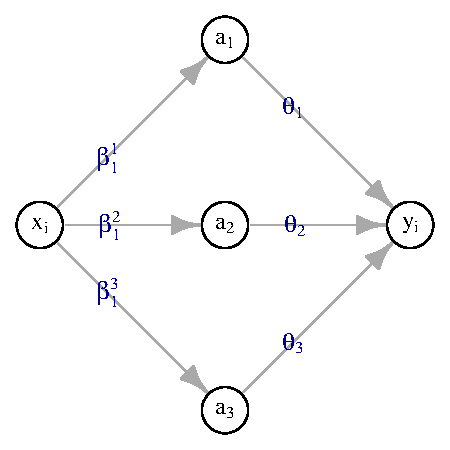
\includegraphics[width=0.5\textwidth]{plot_ANN_01.pdf}
    \caption{Diagram of a multilayer perceptron with $m = 3$.}
    \label{fig:theory_ANN_diagram_01}
\end{figure}

If the response variable $y$ happened to be a categorical variable, let's say binary, then one last transformation would have to be applied to map the model to the $\left[0, 1\right]$ interval and model $y$ as a probability. Then we would have

$$
  y_i =
  \phi \left( \theta_0^{[1]} +  \sum_{j = 1}^m \theta_j^{[1]} \sigma \left( \theta_0^{[0]} + \theta_j^{[0]} x_i \right) \right) =
  \phi \left( \theta_0^{[1]} +  \sum_{j = 1}^m \theta_j^{[1]} a_{j,i} \right),
$$

with $\phi(\cdot)$ the logistic function to map from $\mathbb{R}$ to $\left[ 0, 1 \right]$. The choice of function $\phi(\cdot)$ depends on the nature of the response variable. As we saw previously, in the case of a continuous response variable, $\phi(\cdot)$ is the identity function.

We can establish a more complex model by taking linear combinations of non-linear functions of the previous result. Let's define
$$
a_{k,i}^{[1]} = \sigma^{[1]} \left( \theta_{0}^{[1]} + \theta_k^{[0]} x_i \right)
$$

for $k \in \left\{ 1, \ldots, m \right\}$ and

$$
  a_{k,i}^{[2]} = \sigma^{[2]} \left(  \theta_{0,k}^{[1]} + \sum_{j = 1}^m \theta_{j,k}^{[1]} a_{j,1}^{[0]}  \right)
$$

% $$
% a_{k,i}^{[2]} = \theta_0^{j} +  \sum_{k = 1}^m \theta_k^{j} \sigma^{[2)} \left( \theta_0^{k} + \theta_1^{k} x_i \right) =
% \theta_0^{j} +  \sum_{k = 1}^m \theta_k^{j} a_{k,i}^{[1]}
% $$

for $k \in \left\{ 1, \ldots, r \right\}$, then

$$
  y_i = \theta_0^{[2]} + \sum_{j = 1}^r \theta_j^{[2]} a_{j,i}^{[2]}
$$

where $r$, like $m$, is chosen beforehand. The values $m$ and $r$ are usually called the number of nodes or units of each layer. This is what is called a deeper model, because it has more layers. Notice that we have two different activation functions $\sigma^{[1]}(\cdot)$ and $\sigma^{[2]}(\cdot)$. Each layer can have a different function. The first one could be a sigmoid function and the second one a hyperbolic tangent, or vice versa, or they could both be the same function.

Figure \ref{fig:theory_ANN_diagram_02} shows this graphically with $m = 3$ and $r = 2$. Layers corresponding to $a_{k,i}^{[1]}$ for $k \in \left\{ 1, \ldots, m \right\}$ and $a_{k,i}^{[2]}$ for $k \in \left\{ 1, \ldots, r \right\}$ are called the \textbf{hidden layers}. So figure \ref{fig:theory_ANN_diagram_01} shows a multilayer perceptron with one hidden layer, and figure \ref{fig:theory_ANN_diagram_02} shows a multilayer perceptron with two hidden layers.


\begin{figure}[H]
    \centering
    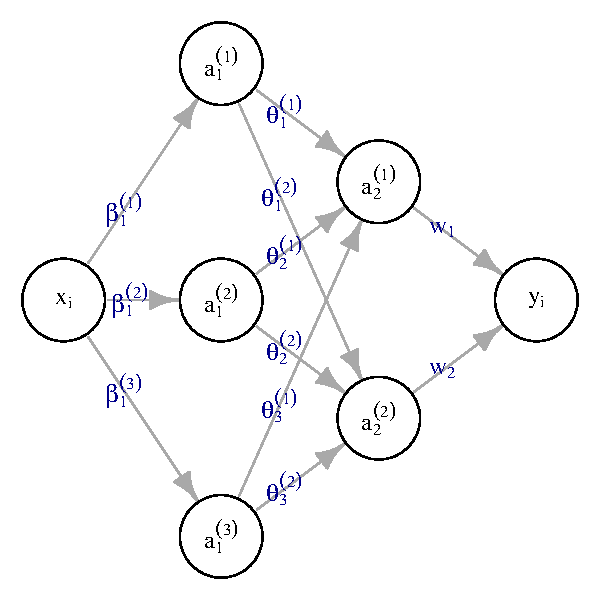
\includegraphics[width=0.6\textwidth]{plot_ANN_02.pdf}
    \caption{Diagram of a multilayer perceptron with two hidden layers, $m = 3$ and $r = 2$.}
    \label{fig:theory_ANN_diagram_02}
\end{figure}

Now that we have a grasp of how the MLP works, we can define it more generally. The notation used will be $y$ for the response variable $n$-dimensional vector, $y_i$ for the $i$-th element of $y$ and $X$ for the data matrix, such that $X \in \mathbb{R}^{n \times p}$, $x_i \in \mathbb{R}^p$ denotes the $i$-th row in $X$ and it represents the values of the covariates for the $i$-th element in the data and $x^{(k)} \in \mathbb{R}^n$ denotes the $k$-th column in $X$ and $x_i^{(k)}$ denotes the $k$-th column-wise element and the $i$-th row-wise element. Since a multilayer perceptron can have any integer number of hidden layers, we will denote the number of layers by $L$, the number of nodes of each layer $l$ by $n^{[l]}$ and the activation function for each layer $l$ by $\sigma^{[l]}(\cdot)$, for $l \in \left\{ 1, \ldots, L \right\}$. The activation function for the last layer will be denoted by $\phi(\cdot)$, as in the binary classification example. The parameter, or weight, that connects the $j$-th node from the $(l-1)$-th layer with the $k$-th node in the $l$-th layer is denoted by $\theta_{j,k}^{[l]}$ and, as before, $a_{k,i}^{[l]}$ denotes the result of the activation function corresponding to the $l$-th layer and the $i$-th observation, for $k \in \left\{ 1, \ldots, n^{[l]} \right\}$; where $\theta_{0,k}^{[l]}$ is the bias term of the $k$-th node in the $l$-th layer. That is,

\begin{equation}
  \label{eq:ann_act_funct_def}
  a_{k,i}^{[l]} = \sigma^{[l]} \left( \theta_{0,k}^{[l-1]} + \sum_{j = 1}^{n^{[l-1]}} \theta_{j,k}^{[l-1]} a_{j,i}^{[l-1]} \right)
\end{equation}

for $k \in \left\{ 1, \ldots, n^{[l]} \right\}$, $j \in \left\{ 1, \ldots, n^{[l-1]} \right\}$, $l \in \left\{ 1, \ldots, L \right\}$ and $i \in \left\{ 1, \ldots, n \right\}$.

To be consistent, $a_{k,i}^{[0]}$ is defined as $x_i^{[k]}$, and so, $a_{k}^{[0]} = x^{(k)} \in \mathbb{R}^n$; and $a_{0,i}^{[0]} = 1$ for all $i \in \left\{ 1, \ldots, n \right\}$, so $a_{0}^{[0]}$ is a vector of ones of dimension $n$ and $n^{[0]}$ is the number of covariates, i.e., $n^{[0]} = p$.

So, in general, a feed-forward neural network or multilayer perceptron with $L$ hidden layers is such that

$$
  y_i = \phi \left( \theta_{0,1}^{[L]} +  \sum_{j = 1}^{n^{[L]}} \theta_{j,1}^{[L]} a_{k,i}^{[L]} \right),
$$

and where equation \ref{eq:ann_act_funct_def} holds. As a way to summarize the whole notation, we will denote a multilayer perceptron with parameters $\Theta$ and data matrix $X$ as $\mathrm{MLP} \left(X, \Theta \right)$, where parameter $\Theta$ is a general way to refer to all parameters $\theta_{j,k}^{[l]}$ for $k \in \left\{ 1, \ldots, n^{[l]} \right\}$, $j \in \left\{ 1, \ldots, n^{[l-1]} \right\}$ and $l \in \left\{ 1, \ldots, L \right\}$.

Figure \ref{fig:theory_ANN_diagram_03} shows an example of an architecture with 2 hidden layers ($L = 2$), 4 covariates ($p = n^{[0]} = 4$), 3 nodes in the first hidden layer ($n^{[1]} = 3$) and 4 nodes in the second hidden layer ($n^{[2]} = 4$).

\begin{figure}[H]
    \centering
    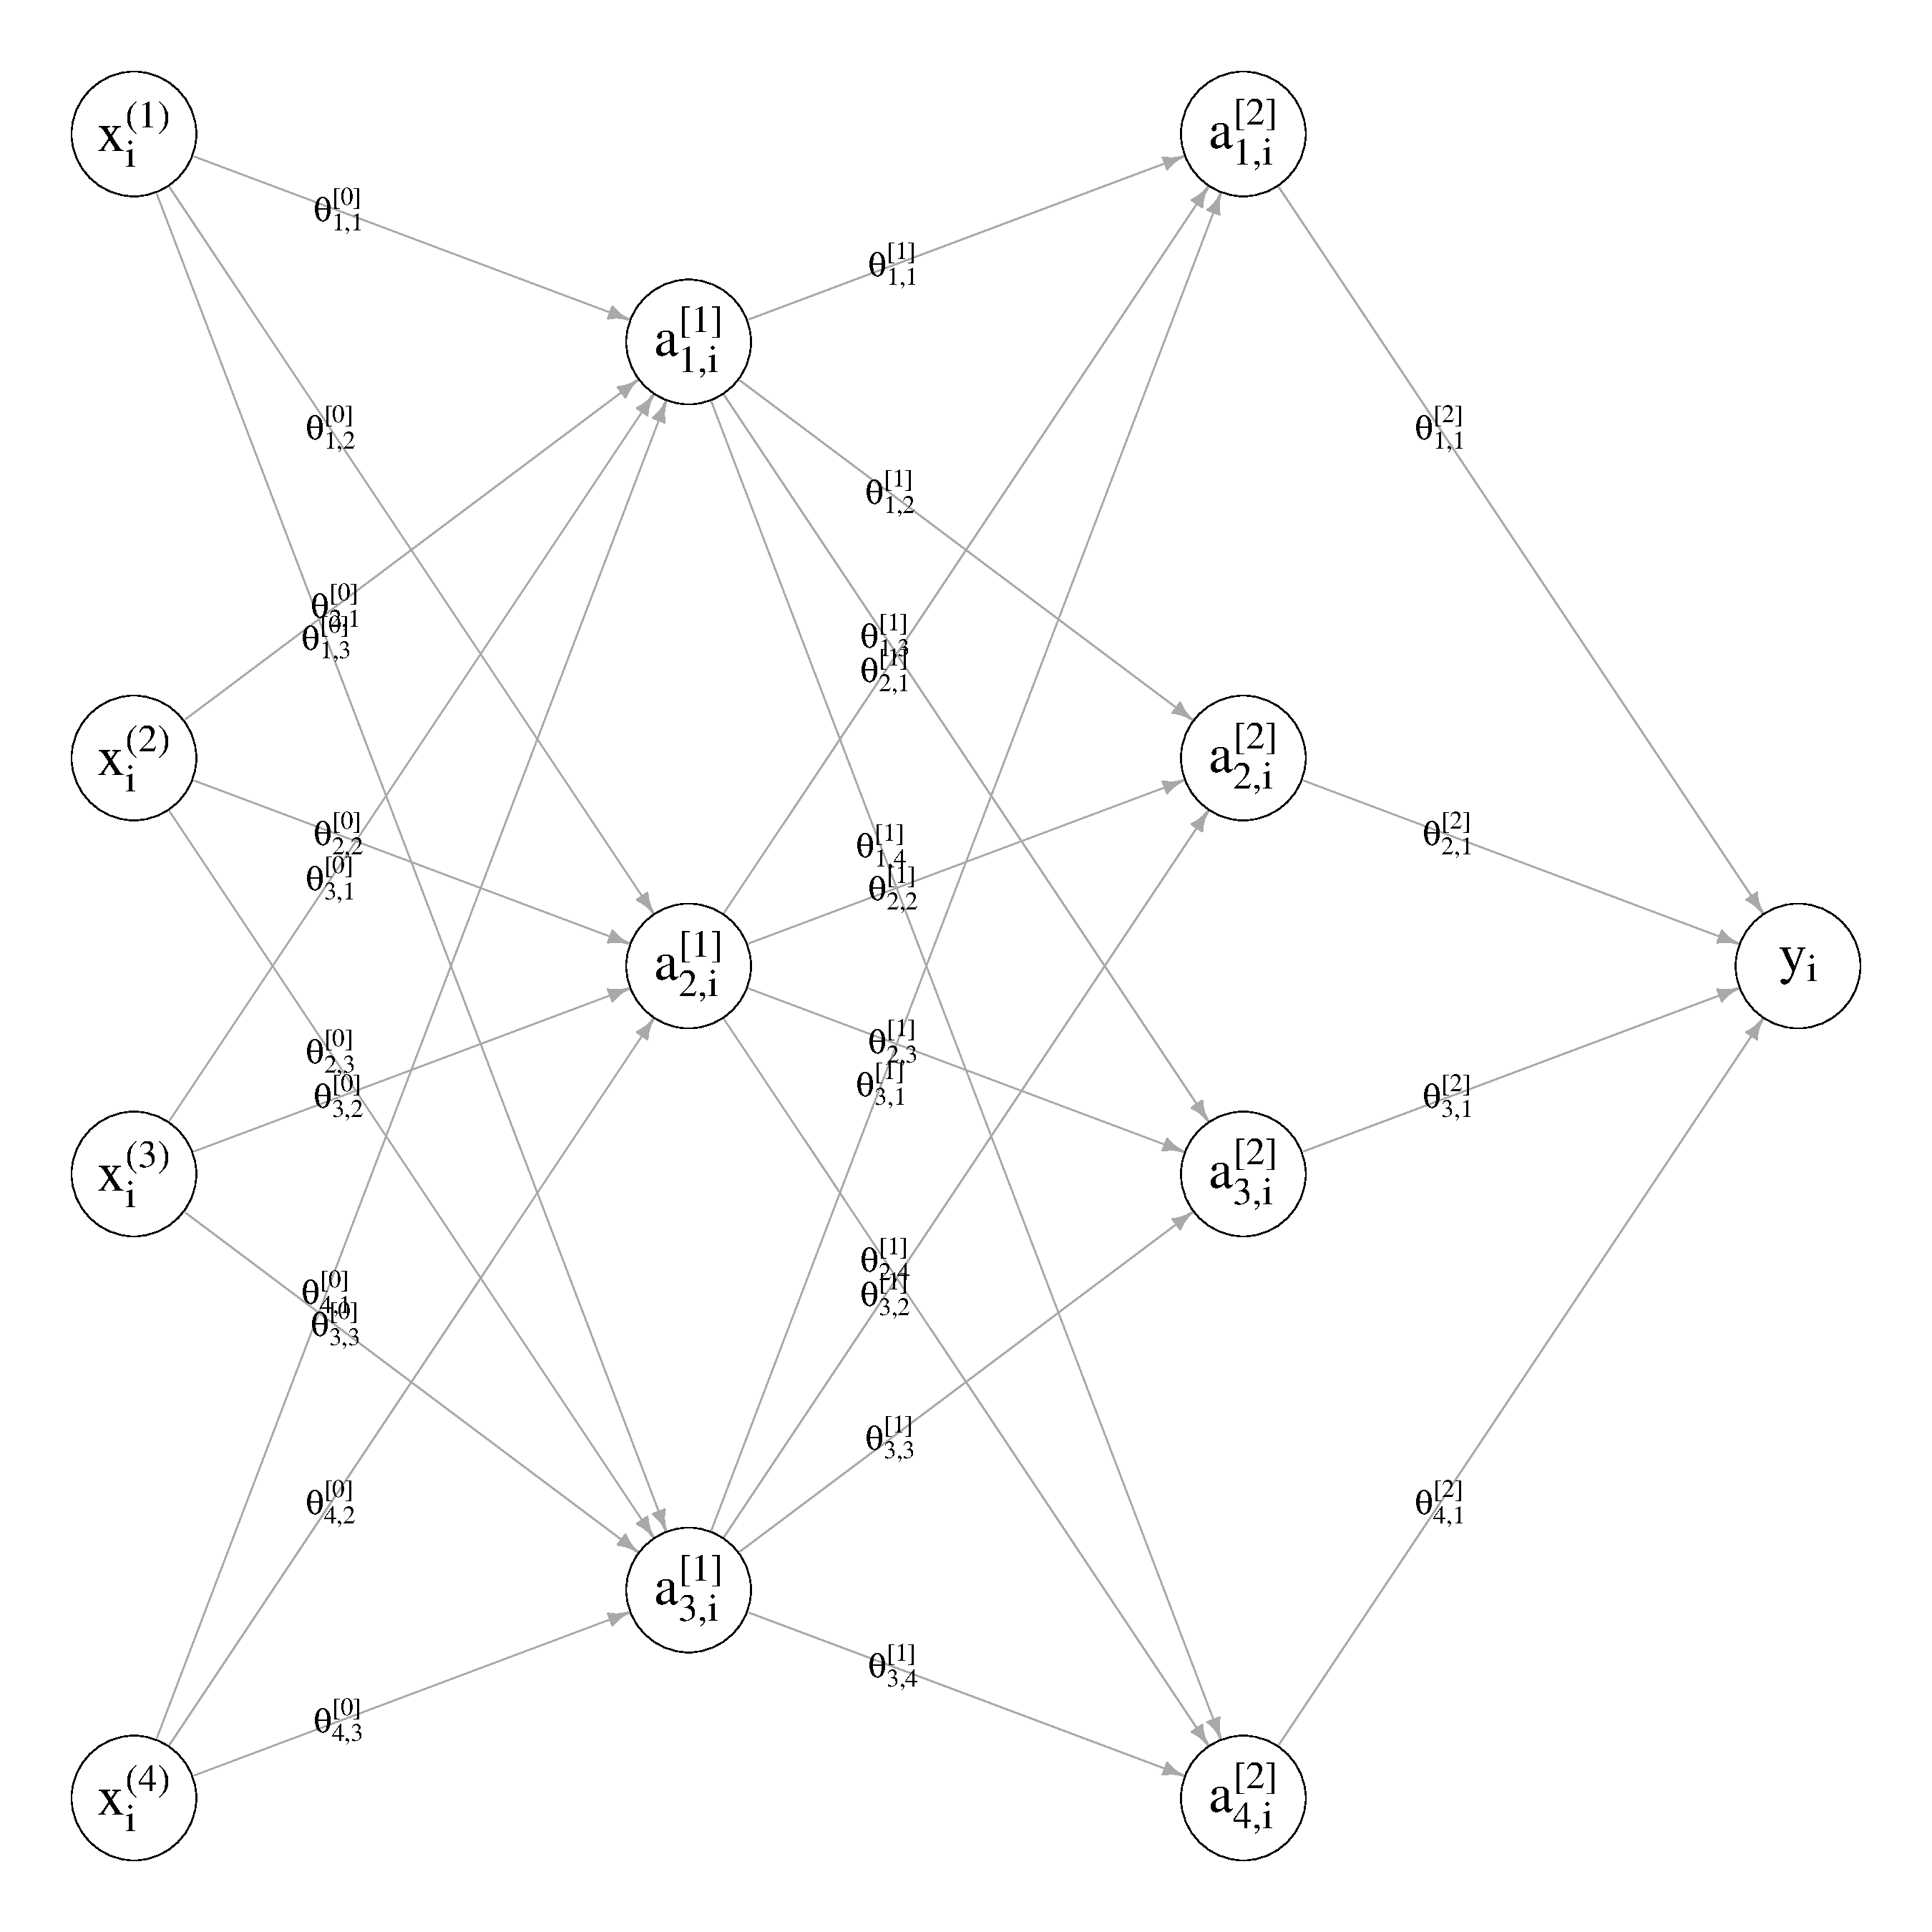
\includegraphics[width=0.95\textwidth]{plot_ANN_03.pdf}
    \caption{Diagram of a multilayer perceptron with two hidden layers using the general notation with $L = 2$, $p = n^{[0]} = 4$, $n^{[1]} = 3$ and $n^{[2]} = 4$.}
    \label{fig:theory_ANN_diagram_03}
\end{figure}

As mentioned before, the values of the parameters in the network are chosen so that they minimize a certain error function. In the continuous case, the commonly called \textbf{squared loss} is often used, defined as the sum of the squared difference between the real values and the output of the model, which is also equivalent to the maximization of a Gaussian likelihood function. This loss function is mathematically defined as

\begin{equation*}
  L(\Theta) = \sum_{i = 1}^n \left[ y_i - \hat{y}_i \right]^2
\end{equation*}

where $\hat{y_i}$ is the output of the model for the $i$-th observation of the data and the covariate vector $x_i$ and $\Theta$ is the vector of all parameters in the model.

In the case of a binary classification problem, a very commonly used loss is the so-called \textbf{cross-entropy} loss, which is the result of maximizing the log-likelihood of independent Bernoulli response variables. In the context of loss function, it is defined as

\begin{equation}
  \label{eq:binary_cross_entropy_loss}
  L(\Theta) = - \sum_{i = 1}^n \left[ y_i \log{\left( \hat{y}_i \right)} + (1 - y_i) \log{\left( 1 - \hat{y}_i \right)} \right].
\end{equation}

In the case of a multiple classification problem, equation \ref{eq:binary_cross_entropy_loss} is extended for more classes using the same maximum likelihood idea. In a $k$ class classification problem, the loss is defined as

\begin{equation*}
  L(\Theta) = - \sum_{i = 1}^n \left[ \sum_{j = 1}^k y_{i,j} \log{\left( \hat{y}_{i,j} \right)}  \right]
\end{equation*}

where $y_{i,j} = 1$ if the $i$-th training point belongs to the $j$-th class and $\hat{y}_{i,j}$ is the model's predicted probability of the $i$-th training point belonging to the $j$-th class.

In the Bayesian approach, we first assign prior distributions to each of the parameters and specify a conditional distribution to the response variable $y$. For example, in the continuous case, it is common to assign a Gaussian conditional distribution to $y$, such that
$$
  y | \Theta, X \sim \normaldist{\mathrm{MLP}(X, \Theta)}{\sigma^2}
$$

where $\mathrm{MLP}(X, \Theta)$ denotes the architecture of a multilayer perceptron with parameters $\Theta$ and data matrix $X$. Since the $\Theta$ parameters can be any real value, it is also common to assign a Gaussian distribution to them, so that the prior distribution is such that

$$
  \theta_{i,k}^{[l]} \sim \normaldist{\mu_{i,k}^{[l]}}{\sigma_{i,k}^{[l]}}.
$$

Parameters $\mu_{i,k}^{[l]}$ and $\sigma_{i,k}^{[l]}$ are chosen to reflect the prior knowledge that we may have about the values of the parameters $\theta_{i,k}^{[l]}$. If we have no prior knowledge, then a vague prior can be used.

In contrast to classical neural networks where parameters $\Theta$ are chosen so that they minimize an error function, in Bayesian neural networks we wish to update our knowledge on the parameters $\Theta$ given the data $X$. This is achieved with Bayes' theorem in the following way

$$
  \prob{\Theta | X} = \frac{\prob{X | \Theta} \prob{\Theta}}{\prob{X}}.
$$

%In our example, $\prob{X | \Theta} = \normalfunc{X}{\mathrm{MLP}(X, \Theta)}{\sigma^2}$ and $\prob{\Theta} = \normalfunc{\Theta}{[]}$
In our example, $\prob{X | \Theta}$ and $\prob{\Theta}$ are the joint density functions of Gaussian random variables with their corresponding parameter values.

To make predictions in the Bayesian case, we use the \textbf{posterior predictive distribution}, defined as

$$
  \prob{x^* | X} = \int \prob{x^* | \Theta} \prob{\Theta | X} \mathrm{d}\Theta
$$

for a new vector of covariates $x^*$.


%%%%%%%%%%%%%%%%%%%%%%%%%%%%%%%%%%%%%%%%%%%%%%%%%%%%%%%%%%%%%%%%%%%%%%%%%%%%%%%%%%%%%%%%%%
%%%%%%%%%%%%%%%%%%%%%%%%%%%%%%%%%%%%%%%%%%%%%%%%%%%%%%%%%%%%%%%%%%%%%%%%%%%%%%%%%%%%%%%%%%
%%% CNNs
%%%%%%%%%%%%%%%%%%%%%%%%%%%%%%%%%%%%%%%%%%%%%%%%%%%%%%%%%%%%%%%%%%%%%%%%%%%%%%%%%%%%%%%%%%
%%%%%%%%%%%%%%%%%%%%%%%%%%%%%%%%%%%%%%%%%%%%%%%%%%%%%%%%%%%%%%%%%%%%%%%%%%%%%%%%%%%%%%%%%%

\section{Convolutional Neural Networks}

Convolutional Neural Networks (CNNs) are neural networks with a quite particular architecture and are widely used in computer vision problems, such as image classification or object detection in a video. They were introduced by \citeauthor{lecun1989generalization} in \citeyear{lecun1989generalization} as a way to constrain the number of parameters needed to perform automatic image classification \cite{lecun1989generalization}. The main idea is that in images, pixels close to each other tend to be similar, whereas pixels far away from each other tend to be different. This notion of proximity is used by CNN's architecture, and leverages three concepts: sparse interactions, parameter sharing and equivariant representations \cite[p.~335]{bengio2015deep}.

\begin{itemize}
  \item Sparse interactions: In MLPs, every unit is connected to all other units in the next layer, but in CNNs, only a small number of units is connected to another small number of units. This means fewer parameters and, hence, less memory usage and faster computation.
  \item Parameter sharing: Different units share the same set of parameters. The same convolution is used many times in the image and, thus, the number of parameters is further reduced.
  \item Equivariant representations: The architecture of CNNs provides equivariance in translations, meaning that if the input is changed, the output is changed in the same fashion. For example: in an image, if an object is moved in the input, its representation will be moved in the same way in the output.
\end{itemize}

\subsection{Convolution operation}

The base of CNNs is the convolution operation, which will be described assuming an image. Let's assume that we have an image represented as a $m \times n$ matrix $I$, with $I_{i,j}$ represents the pixel in the $i$-th row and $j$-th column as such

$$
  I = 
    \begin{bmatrix}
      I_{1,1} & I_{1,2} & I_{1,3} & \dots  & I_{1,n} \\
      I_{2,1} & I_{2,2} & I_{2,3} & \dots  & I_{2,n} \\
      \vdots & \vdots & \vdots & \ddots & \vdots \\
      I_{m,1} & I_{m,2} & I_{m,3} & \dots  & I_{m,n}
    \end{bmatrix}.
$$

The convolution operation uses another matrix called a \textbf{filter} or a \textbf{kernel}, with dimensions $p \times r$. This matrix must be of a lower dimension than the image, that is, $p < m$ and $r < n$. Let's denote the filter as matrix $K$ as such

$$
  K = 
    \begin{bmatrix}
      \theta_{1,1} & \theta_{1,2} & \theta_{1,3} & \dots  & \theta_{1,q} \\
      \theta_{2,1} & \theta_{2,2} & \theta_{2,3} & \dots  & \theta_{2,q} \\
      \vdots & \vdots & \vdots & \ddots & \vdots \\
      \theta_{p,1} & \theta_{p,2} & \theta_{p,3} & \dots  & \theta_{p,q}
    \end{bmatrix}.
$$

The convolution operation between $I$ and $K$ is denoted as $I * K$, and its result is another matrix $S$, for which each element is defined as

\begin{equation}
  \label{eq:2d_conv_def}
  S_{i,j} = (I * K)_{i,j} = \sum_{k} \sum_{l} I_{i+k-1,j+l-1} K_{k, l}.
\end{equation}

An example of this is shown in figure \ref{fig:conv_example}, in which $I$ is a $7 \times 7$ image matrix and the kernel is a $3 \times 3$ matrix. The result is a $5 \times 5$ matrix in which element is computed using equation \ref{eq:2d_conv_def}. For instance, the element on the first row and fourth column of the result matrix, that is, $S_{1,4}$ is computed as 

\begin{equation}
  \begin{split}
      S_{1,4} & = 
      \sum_{k=1}^3 \sum_{l=1}^3 I_{1+k-1,4+l-1} K_{k, l} \\
      & = I_{1,4}K_{1,1} + I_{1,5}K_{1,2} + I_{1,6}K_{1,3} \\
      & + I_{2,4}K_{2,1} + I_{2,5}K_{2,2} + I_{2,6}K_{2,3} \\
      & + I_{3,4}K_{3,1} + I_{3,5}K_{3,2} + I_{3,6}K_{3,3} \\
      & = ( 1 \times 1 ) + ( 0 \times 0 ) + ( 0 \times 1 ) \\
      & + ( 1 \times 0 ) + ( 1 \times 1 ) + ( 0 \times 0 ) \\
      & + ( 1 \times 1 ) + ( 1 \times 0 ) + ( 1 \times 1 ) \\
      & = 4.
  \end{split}
\end{equation}

The rest of the elements are computed in a similar way. Note that the resulting matrix is smaller than the original image matrix. Also note, that the convolution kernel in the example only has 9 parameters which are used by the whole image matrix, and these parameters are usually estimated with data. 

Note that an image classification problem could be solved by turning the input image into a long vector, but then this would be fed to a fully connected layer, which would mean that a large number of parameters would have to be fit. This is one of the reason convolutions are used: instead of estimating a large number of parameters, the convolution operation needs a small number of parameters (9 in the case of the example) to be fit. Additionally, the convolution operation takes into account the topology of the image input, which have a very local structure \cite{lecun1998gradient}.

% $$
%   S_{1,4} = \sum_{k=1}^3 \sum_{l=1}^3 I_{1+k-1,4+l-1} K_{k, l} = I_{1,4}K_{1,1} + I_{1,5}K_{1,2} + I_{1,6}K_{1,3} + I_{2,4}K_{2,1} + I_{2,5}K_{2,2} + I_{2,6}K_{2,3} + I_{3,4}K_{3,1} + I_{3,5}K_{3,2} + I_{3,6}K_{3,3}
% $$

\begin{figure}[H]
    \centering
    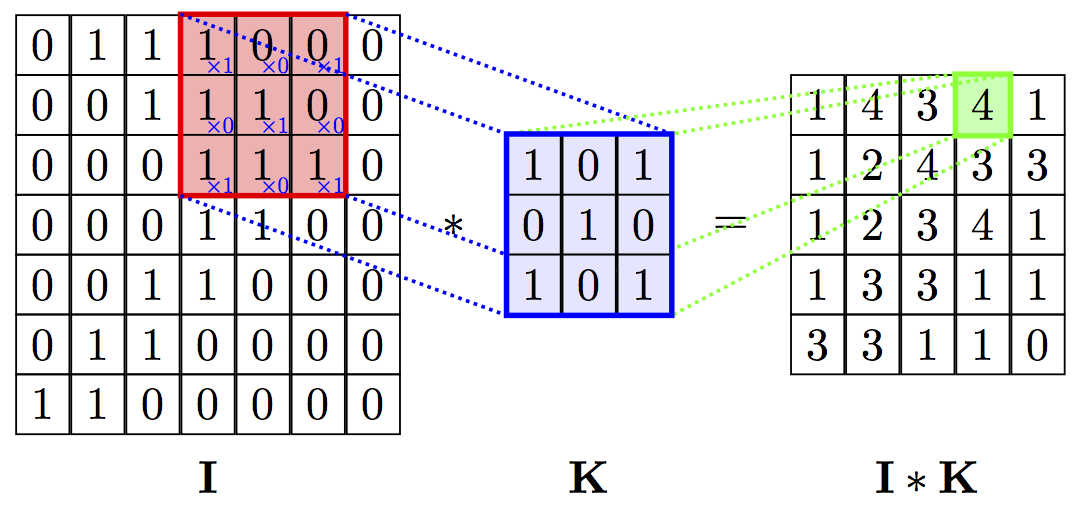
\includegraphics[width=0.9\textwidth]{convolution_example.png}
    \caption{Example of a convolution operation. Source: \url{https://github.com/PetarV-/TikZ}}
    \label{fig:conv_example}
\end{figure}

\subsection{Pooling}

When using CNNs, a pooling layer is also usually added after each convolutional layer. This pooling layer summarizes adjacent pixels, and it is used because it helps to achieve invariance and reduce the image of the output so that there are fewer parameters in the next layers \cite{bengio2015deep}. A very commonly used pooling function is \textbf{max pooling}, which returns the maximum value of a neighborhood of pixels. An example of max pooling is shown in figure \ref{fig:max_pool_example} for a $4 \times 4$ matrix, resulting in a $2 \times 2$ matrix after the function is applied.

\begin{figure}[H]
    \centering
    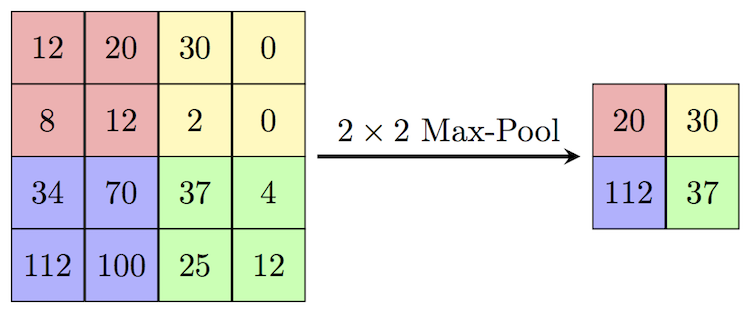
\includegraphics[width=0.6\textwidth]{max_pool_example.png}
    \caption{Example of max pooling function. Source: \url{https://computersciencewiki.org/index.php/File:MaxpoolSample2.png}}
    \label{fig:max_pool_example}
\end{figure}


\subsection{Architecture example}

To illustrate how all these concepts are put together, we will show an example of an architecture that is very commonly used in image classification problems, called \textbf{LeNet architecure}, introduced by \citeauthor{lecun1998gradient} in \citeyear{lecun1998gradient} for a digit classification problem \cite{lecun1998gradient}. The architecture assumes a grayscale input image of $32 \times 32$ pixels, which is then fed to 6 convolutional filters of size $5 \times 5$, each followed by an activation function and a $2 \times 2$ max pooling layer, then 16 convolutional filters of size $5 \times 5$, each with their corresponding activation functions and then the $2 \times 2$ max pooling layer, followed by two fully connected layers of sizes 120 and 84, and finally a softmax transformation to map to the 10 digit classification problem probabilities. 

\begin{figure}[H]
    \centering
    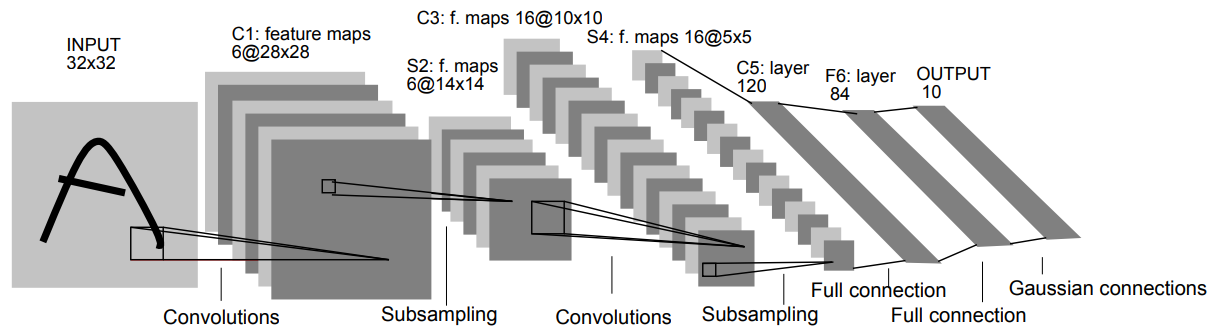
\includegraphics[width=\textwidth]{lenet.png}
    \caption{LeNet architecture (picture taken from \cite{lecun1998gradient}). The feature maps correspond to the convolutional filters and the subsampling refers to max pooling.}
    \label{fig:lenet_architecture}
\end{figure}



%%%%%%%%%%%%%%%%%%%%%%%%%%%%%%%%%%%%%%%%%%%%%%%%%%%%%%%%%%%%%%%%%%%%%%%%%%%%%%%%%%%%%%%%%%
%%%%%%%%%%%%%%%%%%%%%%%%%%%%%%%%%%%%%%%%%%%%%%%%%%%%%%%%%%%%%%%%%%%%%%%%%%%%%%%%%%%%%%%%%%
%%% VI
%%%%%%%%%%%%%%%%%%%%%%%%%%%%%%%%%%%%%%%%%%%%%%%%%%%%%%%%%%%%%%%%%%%%%%%%%%%%%%%%%%%%%%%%%%
%%%%%%%%%%%%%%%%%%%%%%%%%%%%%%%%%%%%%%%%%%%%%%%%%%%%%%%%%%%%%%%%%%%%%%%%%%%%%%%%%%%%%%%%%%

\section{Variational Inference}

As mentioned before, when doing Bayesian inference, it is of interest to compute the posterior distribution $\prob{\theta | X}$, which is very often intractable, so one must resort to numerical approximations. In this section, we'll give a brief overview of one possible numerical approximation, called variational inference (VI). The idea of VI is to use optimization to approximate the target distribution $\prob{\theta | X}$ with some other approximate distribution $q(\theta)$ that minimizes the Kullback-Leibler (KL) divergence to the real posterior \cite{blei2017variational}. We will define such divergence as 
\begin{equation}
  \label{eq:kl_divergence}
  \kl{q}{p} = \mathbb{E}_q \left[ \log \left( \frac{q(\theta)}{\prob{\theta | X}} \right) \right] = \int_{-\infty}^{\infty} q(\theta) \left[ \log \left( \frac{q(\theta)}{\prob{\theta | X}} \right) \right] d\theta.
\end{equation}

Note that the KL divergence is not symmetrical, i.e., $\kl{q}{p} \neq \kl{p}{q}$, and that we usually try to minimize $\kl{q}{p}$ instead of $\kl{p}{q}$ because the latter requires knowing $\prob{\theta | X}$, which is what we are trying to approximate in the first place.

Although the main goal of VI methods is tho minimize the KL divergence in \ref{eq:kl_divergence}, in practice what is usually done is to maximize a related quantity called the ELBO (Evidence Lower BOund), defined as

\begin{equation}
  \label{eq:elbo_def}
  \mathcal{L}(q) = \mathbb{E}_q\left[ \log p(X, \theta) \right] - \mathbb{E}_q\left[ \log q(\theta) \right].
\end{equation}

The relationship between ELBO and KL divergence is easy to see. Starting from the KL divergence definition, using the logarithm quotient rule, and by the fact that the expected value is a linear operator, we have

$$
    \kl{q}{p} = 
    \mathbb{E}_q \left[ \log \left( \frac{q(\theta)}{\prob{\theta | X}} \right) \right] =
    \mathbb{E}_q \left[ \log  q(\theta) \right] - \mathbb{E}_q \left[ \log {\prob{\theta | X}}  \right].
$$

Then, using the definition of conditional probability, we have

$$
    \mathbb{E}_q \left[ \log  q(\theta) \right] - \mathbb{E}_q \left[ \log p(\theta | X)  \right] =
    \mathbb{E}_q \left[ \log  q(\theta) \right] - \mathbb{E}_q \left[ \log \frac{p(\theta, X)}{p(X)}  \right].
$$

Using the logarithm quotient rule one more time

$$
  \mathbb{E}_q \left[ \log  q(\theta) \right] - \mathbb{E}_q \left[ \log \frac{p(\theta, X)}{p(X)}  \right] =
  \mathbb{E}_q \left[ \log  q(\theta) \right] - \mathbb{E}_q \left[ \log p(\theta, X) - \log p(X)  \right].
$$

But since $p(X)$ does not depend on $q$, the expected value of $p(X)$ is a constant; so we have

$$
 \mathbb{E}_q \left[ \log  q(\theta) \right] - \mathbb{E}_q \left[ \log p(\theta, X) - \log p(X)  \right] = 
 \mathbb{E}_q \left[ \log  q(\theta) \right] - \mathbb{E}_q \left[ \log p(\theta, X) \right] + \log p(X).
$$

And since we are trying to find the optimal $q$, then $ļog p(X)$ is just a constant in the optimization process, and we can disregard it and just minimize equation

$$
  \mathbb{E}_q \left[ \log  q(\theta) \right] - \mathbb{E}_q \left[ \log p(\theta, X) \right] 
$$

which as we see, is the negative of the ELBO, so minimizing the KL divergence is equivalent to maximizing the ELBO.


%%%%%%%%%%%%%%%%%%%%%%%%%%%%%%%%%%%%%%%%%%%%%%%%%%%%%%%%%%%%%%%%%%%%%%%%%%%%%%%%%%%%%%%%%%
%%%%%%%%%%%%%%%%%%%%%%%%%%%%%%%%%%%%%%%%%%%%%%%%%%%%%%%%%%%%%%%%%%%%%%%%%%%%%%%%%%%%%%%%%%
%%% AL
%%%%%%%%%%%%%%%%%%%%%%%%%%%%%%%%%%%%%%%%%%%%%%%%%%%%%%%%%%%%%%%%%%%%%%%%%%%%%%%%%%%%%%%%%%
%%%%%%%%%%%%%%%%%%%%%%%%%%%%%%%%%%%%%%%%%%%%%%%%%%%%%%%%%%%%%%%%%%%%%%%%%%%%%%%%%%%%%%%%%%

\section{Active Learning}
